\chapter{\'Evaluation des Mod\`eles}
\label{ch:evaluation}

\section{M\'etriques de classification}
\label{sec:metriques_classif}

\index{exactitude}\index{pr\'ecision}\index{rappel}\index{F1-score}

\begin{definition}[Matrice de confusion]
\index{matrice de confusion}
La \textbf{matrice de confusion} r\'esume les pr\'edictions d'un classifieur binaire en quatre cat\'egories~:
\begin{itemize}
    \item \textbf{Vrais positifs} (VP / TP)~: correctement pr\'edits positifs.
    \item \textbf{Faux positifs} (FP)~: incorrectement pr\'edits positifs (erreur de type I).
    \item \textbf{Vrais n\'egatifs} (VN / TN)~: correctement pr\'edits n\'egatifs.
    \item \textbf{Faux n\'egatifs} (FN)~: incorrectement pr\'edits n\'egatifs (erreur de type II).
\end{itemize}
\end{definition}

\begin{center}
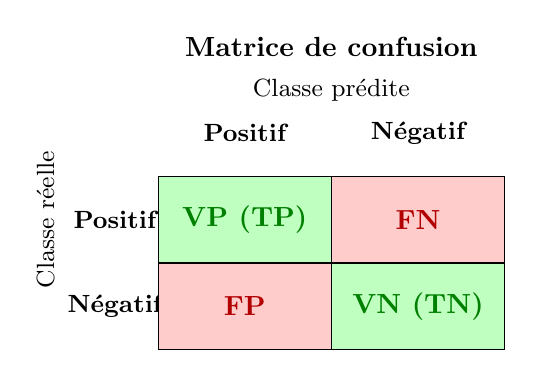
\begin{tikzpicture}[scale=1.1]
    % Titre
    \node[font=\bfseries] at (2.5, 3.5) {Matrice de confusion};
    \node[font=\small, rotate=90] at (-0.8, 1.5) {Classe r\'eelle};
    \node[font=\small] at (2.5, 3) {Classe pr\'edite};

    % En-t\^etes
    \node[font=\small\bfseries] at (1.5, 2.5) {Positif};
    \node[font=\small\bfseries] at (3.5, 2.5) {N\'egatif};
    \node[font=\small\bfseries] at (0, 1.5) {Positif};
    \node[font=\small\bfseries] at (0, 0.5) {N\'egatif};

    % Cellules
    \fill[green!25] (0.5, 1) rectangle (2.5, 2);
    \draw (0.5, 1) rectangle (2.5, 2);
    \node[font=\bfseries, green!50!black] at (1.5, 1.5) {VP (TP)};

    \fill[red!20] (2.5, 1) rectangle (4.5, 2);
    \draw (2.5, 1) rectangle (4.5, 2);
    \node[font=\bfseries, red!70!black] at (3.5, 1.5) {FN};

    \fill[red!20] (0.5, 0) rectangle (2.5, 1);
    \draw (0.5, 0) rectangle (2.5, 1);
    \node[font=\bfseries, red!70!black] at (1.5, 0.5) {FP};

    \fill[green!25] (2.5, 0) rectangle (4.5, 1);
    \draw (2.5, 0) rectangle (4.5, 1);
    \node[font=\bfseries, green!50!black] at (3.5, 0.5) {VN (TN)};
\end{tikzpicture}
\end{center}

\begin{definition}[M\'etriques de classification]
\`A partir de la matrice de confusion, on d\'efinit~:
\begin{align}
\text{Exactitude (Accuracy)} &= \frac{VP + VN}{VP + VN + FP + FN} \\[6pt]
\text{Pr\'ecision} &= \frac{VP}{VP + FP} \quad \text{(parmi les pr\'edits positifs)} \\[6pt]
\text{Rappel (Recall)} &= \frac{VP}{VP + FN} \quad \text{(parmi les vrais positifs)} \\[6pt]
\text{F1-score} &= 2 \cdot \frac{\text{Pr\'ecision} \times \text{Rappel}}{\text{Pr\'ecision} + \text{Rappel}}
\end{align}
\end{definition}

\begin{intuition}
\begin{itemize}
    \item La \textbf{pr\'ecision} r\'epond \`a~: <<~Parmi ceux que j'ai d\'eclar\'es malades, combien le sont vraiment~? ~>>
    \item Le \textbf{rappel} r\'epond \`a~: <<~Parmi les vrais malades, combien ai-je d\'etect\'es~? ~>>
    \item Le \textbf{F1-score} est la moyenne harmonique des deux, utile quand les classes sont d\'es\'equilibr\'ees.
\end{itemize}
\end{intuition}

\subsection{Exemple avec le Titanic}

\begin{codeblock}[title=\textbf{Python}]
\begin{minted}{python}
import seaborn as sns
import pandas as pd
from sklearn.model_selection import train_test_split
from sklearn.ensemble import RandomForestClassifier
from sklearn.metrics import (classification_report,
                             confusion_matrix, accuracy_score)

# Pr\'eparation des donn\'ees Titanic
titanic = sns.load_dataset('titanic').dropna(subset=['age', 'fare'])
titanic['sex_num'] = titanic['sex'].map({'male': 0, 'female': 1})
X = titanic[['pclass', 'age', 'fare', 'sex_num']]
y = titanic['survived']

X_train, X_test, y_train, y_test = train_test_split(
    X, y, test_size=0.3, random_state=42, stratify=y
)

# Entra\^inement
rf = RandomForestClassifier(n_estimators=100, random_state=42)
rf.fit(X_train, y_train)
y_pred = rf.predict(X_test)

# Matrice de confusion
print("Matrice de confusion :")
print(confusion_matrix(y_test, y_pred))
print()
print("Rapport de classification :")
print(classification_report(y_test, y_pred, target_names=['D\'ec\'ed\'e', 'Survécu']))
\end{minted}
\end{codeblock}

\begin{codeoutput}
\begin{minted}{text}
Matrice de confusion :
[[103  19]
 [ 25  67]]

Rapport de classification :
              precision    recall  f1-score   support

     Décédé       0.80      0.84      0.82       122
     Survécu       0.78      0.73      0.75        92

    accuracy                           0.79       214
   macro avg       0.79      0.79      0.79       214
weighted avg       0.79      0.79      0.79       214
\end{minted}
\end{codeoutput}

\begin{attention}
L'\textbf{exactitude} seule est trompeuse sur des donn\'ees d\'es\'equilibr\'ees. Si 95\% des e-mails sont l\'egitimes, un mod\`ele qui pr\'edit toujours <<~l\'egitime ~>> aura 95\% d'exactitude mais ne d\'etectera aucun spam~!
\end{attention}

\section{Courbe ROC et AUC}
\label{sec:roc_auc}

\index{courbe ROC}\index{AUC}

\begin{definition}[Courbe ROC]
La \textbf{courbe ROC} (\textit{Receiver Operating Characteristic}) trace le \textbf{taux de vrais positifs} (rappel) en fonction du \textbf{taux de faux positifs} pour diff\'erents seuils de d\'ecision. L'\textbf{AUC} (\textit{Area Under the Curve}) mesure l'aire sous cette courbe~: $\text{AUC} \in [0, 1]$.
\end{definition}

\begin{codeblock}[title=\textbf{Python}]
\begin{minted}{python}
from sklearn.metrics import roc_auc_score, roc_curve

# Probabilit\'es pr\'edites
y_proba = rf.predict_proba(X_test)[:, 1]

# AUC
auc = roc_auc_score(y_test, y_proba)
print(f"AUC : {auc:.4f}")

# Points de la courbe ROC
fpr, tpr, thresholds = roc_curve(y_test, y_proba)
print(f"Nombre de seuils : {len(thresholds)}")
print(f"FPR (5 premiers) : {fpr[:5].round(3)}")
print(f"TPR (5 premiers) : {tpr[:5].round(3)}")
\end{minted}
\end{codeblock}

\begin{codeoutput}
\begin{minted}{text}
AUC : 0.8575
Nombre de seuils : 18
FPR (5 premiers) : [0.    0.    0.008 0.016 0.041]
TPR (5 premiers) : [0.    0.011 0.065 0.13  0.239]
\end{minted}
\end{codeoutput}

\begin{remarque}
Un classifieur al\'eatoire a une AUC de $0{,}5$ (diagonale). Un classifieur parfait a une AUC de $1{,}0$. En g\'en\'eral, une AUC $> 0{,}8$ est consid\'er\'ee comme bonne.
\end{remarque}

\section{M\'etriques de r\'egression}
\label{sec:metriques_regression}

\index{MAE}\index{MSE}\index{RMSE}

\begin{definition}[M\'etriques de r\'egression]
Soit $\hat{y}_i$ les pr\'edictions et $y_i$ les valeurs r\'eelles~:
\begin{align}
\text{MAE} &= \frac{1}{n}\sum_{i=1}^{n}|y_i - \hat{y}_i| \\[6pt]
\text{MSE} &= \frac{1}{n}\sum_{i=1}^{n}(y_i - \hat{y}_i)^2 \\[6pt]
\text{RMSE} &= \sqrt{\text{MSE}} \\[6pt]
R^2 &= 1 - \frac{\sum(y_i - \hat{y}_i)^2}{\sum(y_i - \bar{y})^2}
\end{align}
\end{definition}

\begin{codeblock}[title=\textbf{Python}]
\begin{minted}{python}
from sklearn.metrics import mean_absolute_error, mean_squared_error, r2_score
from sklearn.linear_model import LinearRegression
import numpy as np

tips = sns.load_dataset('tips')
X_reg = tips[['total_bill', 'size']]
y_reg = tips['tip']

X_train, X_test, y_train, y_test = train_test_split(
    X_reg, y_reg, test_size=0.3, random_state=42
)

reg = LinearRegression()
reg.fit(X_train, y_train)
y_pred = reg.predict(X_test)

print(f"MAE  : {mean_absolute_error(y_test, y_pred):.4f}")
print(f"MSE  : {mean_squared_error(y_test, y_pred):.4f}")
print(f"RMSE : {np.sqrt(mean_squared_error(y_test, y_pred)):.4f}")
print(f"R\u00b2   : {r2_score(y_test, y_pred):.4f}")
\end{minted}
\end{codeblock}

\begin{codeoutput}
\begin{minted}{text}
MAE  : 0.7359
MSE  : 1.0940
RMSE : 1.0459
R²   : 0.4616
\end{minted}
\end{codeoutput}

\section{Validation crois\'ee avanc\'ee}
\label{sec:cv_avancee}

\index{validation crois\'ee stratifi\'ee}\index{StratifiedKFold}

\begin{definition}[Validation crois\'ee stratifi\'ee]
La \textbf{validation crois\'ee stratifi\'ee}\index{validation crois\'ee stratifi\'ee} pr\'eserve la \textbf{proportion des classes} dans chaque pli. Elle est recommand\'ee pour la classification, surtout avec des classes d\'es\'equilibr\'ees.
\end{definition}

\begin{codeblock}[title=\textbf{Python}]
\begin{minted}{python}
from sklearn.model_selection import cross_val_score, StratifiedKFold

# Validation crois\'ee stratifi\'ee \`a 5 plis
skf = StratifiedKFold(n_splits=5, shuffle=True, random_state=42)

rf = RandomForestClassifier(n_estimators=100, random_state=42)
scores = cross_val_score(rf, X, y, cv=skf, scoring='f1')

print(f"F1-scores par pli : {scores.round(4)}")
print(f"F1 moyen : {scores.mean():.4f} (+/- {scores.std():.4f})")
\end{minted}
\end{codeblock}

\begin{codeoutput}
\begin{minted}{text}
F1-scores par pli : [0.7273 0.7143 0.7500 0.7647 0.7692]
F1 moyen : 0.7451 (+/- 0.0207)
\end{minted}
\end{codeoutput}

\section{Optimisation des hyperparam\`etres}
\label{sec:gridsearch}

\index{GridSearchCV}\index{hyperparam\`etres}

\begin{definition}[GridSearchCV]
\py{GridSearchCV} effectue une \textbf{recherche exhaustive} sur une grille d'hyperparam\`etres, en \'evaluant chaque combinaison par validation crois\'ee.
\end{definition}

\begin{codeblock}[title=\textbf{Python}]
\begin{minted}{python}
from sklearn.model_selection import GridSearchCV
from sklearn.ensemble import RandomForestClassifier

# D\'efinition de la grille
param_grid = {
    'n_estimators': [50, 100, 200],
    'max_depth': [3, 5, 10, None],
    'min_samples_split': [2, 5]
}

grid_search = GridSearchCV(
    RandomForestClassifier(random_state=42),
    param_grid,
    cv=5,
    scoring='accuracy',
    n_jobs=-1
)
grid_search.fit(X_train, y_train)

print(f"Meilleurs param\`etres : {grid_search.best_params_}")
print(f"Meilleur score (CV)  : {grid_search.best_score_:.4f}")
print(f"Score sur le test    : {grid_search.score(X_test, y_test):.4f}")
\end{minted}
\end{codeblock}

\begin{codeoutput}
\begin{minted}{text}
Meilleurs param\`etres : {'max_depth': 5, 'min_samples_split': 5, 'n_estimators': 100}
Meilleur score (CV)  : 0.8006
Score sur le test    : 0.7944
\end{minted}
\end{codeoutput}

\begin{bonnepratique}
Utilisez \py{GridSearchCV} pour trouver les meilleurs hyperparam\`etres de mani\`ere syst\'ematique. Pour de grandes grilles, pr\'ef\'erez \py{RandomizedSearchCV}\index{RandomizedSearchCV} qui \'echantillonne al\'eatoirement un sous-ensemble de combinaisons.
\end{bonnepratique}

\section{Courbes d'apprentissage}
\label{sec:learning_curves}

\index{courbe d'apprentissage}

\begin{definition}[Courbe d'apprentissage]
Une \textbf{courbe d'apprentissage} trace le score d'entra\^inement et de validation en fonction de la \textbf{taille de l'ensemble d'entra\^inement}. Elle permet de diagnostiquer le sur-apprentissage ou le sous-apprentissage.
\end{definition}

\begin{codeblock}[title=\textbf{Python}]
\begin{minted}{python}
from sklearn.model_selection import learning_curve
import numpy as np

train_sizes, train_scores, val_scores = learning_curve(
    RandomForestClassifier(n_estimators=50, random_state=42),
    X, y, cv=5,
    train_sizes=np.linspace(0.1, 1.0, 5),
    scoring='accuracy'
)

print("Taille | Score train | Score valid.")
print("-" * 42)
for size, tr, va in zip(train_sizes, train_scores.mean(axis=1),
                         val_scores.mean(axis=1)):
    print(f"  {size:4d} |    {tr:.4f}   |    {va:.4f}")
\end{minted}
\end{codeblock}

\begin{codeoutput}
\begin{minted}{text}
Taille | Score train | Score valid.
------------------------------------------
    52 |    0.9962   |    0.6930
   104 |    0.9923   |    0.7451
   157 |    0.9936   |    0.7686
   210 |    0.9924   |    0.7851
   263 |    0.9924   |    0.7944
\end{minted}
\end{codeoutput}

\begin{intuition}
\begin{itemize}
    \item Si les scores d'entra\^inement et de validation sont \textbf{proches et bas}~: sous-apprentissage (augmenter la complexit\'e).
    \item Si le score d'entra\^inement est \textbf{\'elev\'e} mais le score de validation est \textbf{bas}~: sur-apprentissage (r\'eduire la complexit\'e ou augmenter les donn\'ees).
    \item Si les deux scores \textbf{convergent vers une valeur \'elev\'ee}~: bon mod\`ele.
\end{itemize}
\end{intuition}

\section{Exercices}

\begin{exercice}[$\star$]
Calculez manuellement la pr\'ecision, le rappel et le F1-score \`a partir de la matrice de confusion suivante~:
\[
\begin{pmatrix} 45 & 5 \\ 10 & 40 \end{pmatrix}
\]
V\'erifiez vos r\'esultats avec scikit-learn.
\end{exercice}

\begin{exercice}[$\star$]
Expliquez dans quel cas on privil\'egie le rappel plut\^ot que la pr\'ecision. Donnez deux exemples concrets.
\end{exercice}

\begin{exercice}[$\star\star$]
Sur le jeu Iris, entra\^inez un KNN et tracez la courbe ROC (one-vs-rest) pour chaque classe. Calculez l'AUC pour chaque classe.
\end{exercice}

\begin{exercice}[$\star\star$]
Utilisez \py{GridSearchCV} pour optimiser les hyperparam\`etres d'un \py{KNeighborsClassifier} sur le jeu de donn\'ees \texttt{penguins} de seaborn. Testez $k \in \{1, 3, 5, 7, 9, 11\}$ et les m\'etriques de distance \py{('euclidean', 'manhattan')}.
\end{exercice}

\begin{exercice}[$\star\star\star$]
Sur le jeu Titanic, comparez trois mod\`eles (r\'egression logistique, for\^et al\'eatoire, KNN) en utilisant la validation crois\'ee stratifi\'ee \`a 10 plis. Pour chaque mod\`ele, rapportez l'exactitude, la pr\'ecision, le rappel et le F1-score moyens. Quel mod\`ele recommandez-vous et pourquoi~?
\end{exercice}

\begin{exercice}[$\star\star\star$]
Tracez les courbes d'apprentissage pour un arbre de d\'ecision avec \py{max_depth=2}, \py{max_depth=5} et \py{max_depth=None} sur le jeu Titanic. Interpr\'etez les r\'esultats en termes de biais-variance.
\end{exercice}

\begin{formules}
\textbf{R\'esum\'e du chapitre~\ref{ch:evaluation}}
\begin{itemize}
    \item \textbf{Matrice de confusion}~: VP, FP, VN, FN.
    \item \textbf{Exactitude}~: $(VP + VN) / N$, trompeuse si classes d\'es\'equilibr\'ees.
    \item \textbf{Pr\'ecision}~: $VP / (VP + FP)$, \textbf{Rappel}~: $VP / (VP + FN)$.
    \item \textbf{F1-score}~: $2 \cdot \frac{\text{Pr\'ecision} \times \text{Rappel}}{\text{Pr\'ecision} + \text{Rappel}}$.
    \item \textbf{Courbe ROC / AUC}~: TPR vs.\ FPR, $\text{AUC} \in [0, 1]$.
    \item \textbf{R\'egression}~: MAE, MSE, RMSE, $R^2$.
    \item \textbf{GridSearchCV}~: recherche exhaustive d'hyperparam\`etres avec CV.
    \item \textbf{Courbe d'apprentissage}~: diagnostic sur-/sous-apprentissage.
\end{itemize}
\end{formules}
